\section{Experiments}

In the following sections we present the results of our experiments. For all simulated data
we generate our response vector according to \(\vec{y} = \mat{X}\vec{\beta}^* +
\vec{\varepsilon},\) with \(\vec{\varepsilon} \sim \normal(\vec{0}, \sigma_\varepsilon^2
\mat{I})\). We consider two types of features: binary (quasi-Bernoulli) and quasi-normal
features. To generate binary vectors, we sample \(\ceil{nq_j}\) indexes uniformly at random
without replacement from \([n]\) and set the corresponding elements to one and the
remaining ones to zero. To generate quasi-normal features, we generate a linear sequence
\(\vec{w}\) with \(n\) values from \(10^{-4}\) to \(1 - 10^{-4}\), set \(x_{ij} =
\cdf^{-1}(w_i)\), and then shuffle the elements of \(\vec{x}_j\) uniformly at random.

We use a coordinate descent solver to optimize our models, which we have based on the
algorithm outlined by \citet{friedman2010}. All experiments were coded using the Julia
programming language~\citep{bezanson2017} and the code is available at
\url{https://github.com/jolars/normreg}. All simulated experiments were run for 50
iterations and, unless stated otherwise, are presented as means $\pm$ one standard
deviation (using bars or ribbons).

\subsection{Normalization in the Lasso and Ridge Regression}%
\label{sec:experiments-lassoridge}

In this section we consider fitting the lasso and ridge regression to normalized data sets.
To normalize the data, we use standardize all quasi-normal features. For binary features,
we center by mean and scale by \(s_j \propto (q_j-q_j^2)^\delta\).
% where \(\delta = 0\)
% corresponds to no scaling, \(\delta = 1/2\) to standardization, and \(\delta = 1\) to
% variance scaling.

\subsubsection{Variability and Bias in Estimates}

In our first experiment, we consider fitting the lasso to a simulated data set with
\(n=500\) observations and \(p = \num{1000}\) features, out of which the first 20 features
correspond to signals, with \(\beta_j^*\) decreasing linearly from 1 to 0.1. We introduce
dependence between the features by copying the first \(\ceil{\rho n/2}\) values from the
first feature to each of the following features. In addition, we set the class balance of
the first 20 features so that it decreases linearly on a log-scale from 0.5 to 0.99. We
estimate the regression coefficients using the lasso, setting \(\lambda_1 = 2
\sigma_\varepsilon \sqrt{2 \log p }\).

The results~(\Cref{fig:binary-decreasing}, and \Cref{fig:binary-decreasing-full} in
\Cref{sec:additional-results-biasvar}) show that class balance has considerable effect,
particularly in the case of no scaling (\(\delta = 0\)), which corroborates our theory from
\Cref{sec:theory-binary-features}. At \(q_j=0.99\), for instance, the estimate
(\(\hat{\beta}_{20}\)) is consistently zero when \(\delta = 0\). For \(\delta=1\), we see
that class imbalance increases the variance of the estimates. What is also clear is that
the variance of the estimates increase with class imbalance and that this effect increases
together with \(\delta\).

\begin{figure}[htpb]
  \centering
  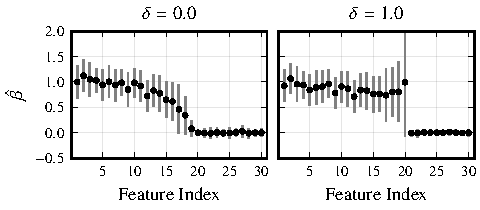
\includegraphics[]{plots/binary_decreasing_small.pdf}
  \caption{%
    Regression coefficients for a lasso problem with binary data where \(n = 500\) and
    \(p = \num{1000}\) with 20 true signals. Here we show only the first 30
    coefficients. See \Cref{sec:experiments-lassoridge} for more information
    on the setup of this experiment.
  }
  \label{fig:binary-decreasing}
\end{figure}

\subsubsection{Predictive Performance}

\textcolor{red}{Our previous results indicate that the choice of normalization matters also for predictive
  performance}, in this section we will examine whether that is the case for three
different data sets: \data{a1a}~\citep{becker1996}, \data{rhee2006}~\citep{rhee2006}, and
\data{w1a}~\citep{platt1998}.\footnote{See \Cref{sec:data-summary} for details about these
  data sets.} We consider performance in terms of normalized mean-squared error~(NMSE) for
lasso and ridge regression across a two-dimensional grid of \(\delta\) and \(\lambda\),
where for \(\delta\) we use a linear sequence from 0 to 1, and for \(\lambda\) a geometric
sequence from \(\lambda_\text{max}\) (the value of \(\lambda\) at which the first feature
enters the model) to \(10^{-2}\lambda_\text{max}\). We split the data into equal training
and validation set splits and for each combination of \(\lambda\) and \(\delta\) fit the
lasso or ridge to the training set.

We present the results for ridge regression in \Cref{fig:hyperopt-contours}, which shows
contour plots of the validation set error. We see that optimal setting of \(\delta\)
differs between the different data sets, suggesting that it is useful to choose \(\delta\)
by hyperparameter optimization. See
\Cref{fig:hyperopt-contours-full}~(\Cref{sec:predictive-performance-simulated}) for a plot
that includes the lasso as well.

% For
% \data{a1a}, the lasso is generally quite insensitive to the type of normalization, even if
% the optimal value is around 0.2. For ridge regression, lower values of \(\delta\) clearly
% work better. With the \data{w1a} data set, however, the relationship is flipped in the case
% of ridge regression and the optimal value is approximately 0.8. In the case of the lasso
% (for \(\data{w1a}\)), a value around 0.5 is optimal and low values (little scaling) yield
% worse prediction errors. Finally, for \data{rhee2006}, the lasso is again insensitive to
% normalization type. This is not the case for ridge, however, where a value around 0.2 is
% optimal and high values of \(\delta\) yield worse prediction errors.

\begin{figure}[htpb]
  \centering
  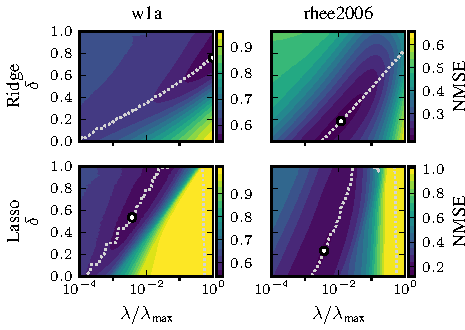
\includegraphics[]{plots/hyperopt_surfaces_small.pdf}
  \caption{%
    Contour plots of normalized validation set mean-squared error (NMSE)
    for \(\delta\) and \(\lambda\) in ridge regression on
    three real data sets. The
    dotted path shows the smallest NMSE as a function of \(\lambda\) and the circles mark
    combinations with the lowest error.
  }
  \label{fig:hyperopt-contours}
\end{figure}

% We would like to point out that there is a dependency between \(\lambda\) and \(\delta\)
% that make it difficult to interpret the relationship between them and the error. This comes
% from the fact that scaling with a smaller value (as in \(\delta = 1\)) increases the sizes
% of the vectors, which means that the level of penalization is relaxed, relatively speaking.

In \Cref{sec:predictive-performance-simulated}, we extend these results with experiments on
simulated data under various class balances and signal-to-noise ratios, again showing that
normalization has an impact on predictive preformance.

\subsubsection{Mixed Data}\label{sec:experiments-mixed-data}

In \Cref{sec:mixed-data} we showed theoretically that care needs to be taken when
normalizing mixed data. Here we verify the theory through simulations. We construct a
quasi-normal feature with mean zero and standard deviation 1/2 and a binary feature with
varying class balance \(q_j\). We set the signal-to-noise ratio to 0.5 and use \(n =
\num{1000}\). These features are constructed so that their effects are comparable under the
notion of comparability that we introduced in \Cref{sec:mixed-data} using \(\kappa = 2\).
In order to preserve the comparability for the baseline case when we have perfect class
balance, we scale by \(s_j = 2 \times (1/4)^{1-\delta}(q_j-q_j^2)^\delta\). Finally, we set
\(\lambda\) to \(\lambda_\text{max}/2\) and \(2\lambda_\text{max}\) for lasso and ridge
regression respectively.

The results~(\Cref{fig:lasso-ridge-comparison}) reflect our theoretical results from
\Cref{sec:theory}. In the case of the lasso, we need \(\delta =1\) (variance scaling) to
avoid the effect of class imbalance, whereas for ridge we instead need \(\delta =1/2\)
(standardization). As our theory suggests, this extra scaling mitigates this class-balance
dependency at the cost of added variance.
% Note that we do not see the bias reduction that
% we observed in our theoretical results for high \(q_j\) values and \(\delta \geq 1/2\) in
% \Cref{fig:lasso-ridge-comparison}. This is related to the error term (signal-to-noise
% ratio) and level of \(q_j\). We would need stronger class imbalance and larger error for
% the effect to show up here.

\begin{figure}[htpb]
  \centering
  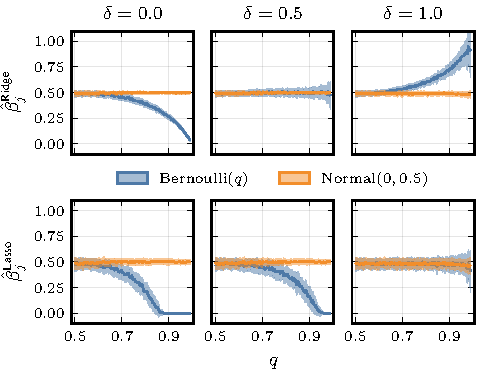
\includegraphics{plots/mixed_data.pdf}
  \caption{%
    Lasso and ridge estimates for a two-dimensional problem where one feature is a binary
    feature with class balance \(q_j\) (\(\bernoulli(q_j)\)) and the other is quasi-normal
    with standard deviation 1/2, (\(\normal(0, 0.5)\)).
  }
  \label{fig:lasso-ridge-comparison}
\end{figure}

\subsubsection{Interactions}\label{sec:experiments-interactions}

Next, we study the effects of normalization and class balance on interactions in the lasso.
Our example consists of a two-feature problem with an added interaction term given by
\(x_{i3} = x_{i1}x_{i2}\). The first feature is binary with class balance \(q\) and the
second quasi-normal with standard deviation 0.5. We use \(n=1000\), \(\lambda_1 = n/4\),
and normalize the binary feature by mean-centering and scaling by \(\kappa (q - q^2)\),
using \(\kappa = 2\). We consider two different strategies for choosing \(s_3\): in the
first strategy, which we call \emph{Strategy 1}, we simply standardize the resulting
interaction feature.
% TODO: make a reference to where this is done
In the second strategy, \emph{Strategy 2} we center with mean and scale with \(s_1s_2\)
(the product of the scales of the binary and normal features).

The results for the case when \(\bm{\beta}^* = \bm{1}\)~(\Cref{fig:interactions}) show that
only strategy 2 estimates the effect of the interaction correctly. Strategy 1, meanwhile,
only selects the correct model if the class balance of the binary feature is close to 1/2
and in general shrinks the coefficient too much. See
\Cref{fig:interactions-full}~(\Cref{sec:additional-experiments-interactions}) for results
on different choices of \(\bm{\beta}^*\).

\begin{figure}[htpb]
  \centering
  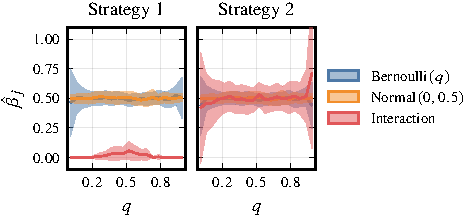
\includegraphics[]{plots/interactions-classbalance-small.pdf}
  \caption{%
    Lasso estimates for a problem with a binary feature, a quasi-normal feature, and
    an interaction feature. We have set \(\bm{\beta}^* = \bm{1}\) and use two different normalization strategies where
    Strategy 1 represents standardization and Strategy 2 is mean-centering
    together with scaling by \(s_1 s_2\).
  }
  \label{fig:interactions}
\end{figure}

\subsection{The Weighted Elastic Net}

The weighted elastic net can be used as an alternative to normalization to correct for
class balance bias when \(\lambda_1 > 0\) and \(\lambda_2 >0\). To simplify the
presentation, we parameterize the elastic net as \(\lambda_1 = \alpha \lambda \) and
\(\lambda_2 = (1-\alpha) \lambda\), so that \(\alpha\) controls the balance between the
ridge and lasso. We conduct an experiment with the same setup as in
\Cref{sec:experiments-mixed-data}, but here we use the weighted elastic net instead with
\(\alpha = 0.5\) (See \Cref{sec:additional-experiments-weighted-elnet} for results using
other setting for \(\alpha\)). We use \(n=1000\) and vary \(\omega\), using the weights
\(u_j = v_j = (q_j - q_j^2)^{\omega}\) as we suggested in \Cref{sec:binary-weighting}. Our
results (\Cref{fig:mixed-data-elnet}) show that \(\omega = 1\) leads to seemingly unbiased
estimates.

\begin{figure}[htpb]
  \centering
  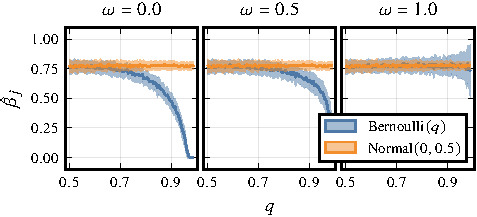
\includegraphics{plots/mixed_data_elnet_small.pdf}
  \caption{%
    Weighted elastic net estimates for \(\alpha = 0.5\) for a problem with a binary
    feature with class balance \(q\) (\(\bernoulli(q)\)) and quasi-normal
    with standard deviation 1/2 (\(\normal(0, 0.5)\)). \(\omega\) indicates
    the scaling of the penalty weights.
  }
  \label{fig:mixed-data-elnet}
\end{figure}

